\documentclass[tikz,border=2pt]{standalone}
\usepackage{pgfplots}
\usetikzlibrary{intersections}
\usepgfplotslibrary{fillbetween}
\pgfplotsset{compat=1.7}

\begin{document}
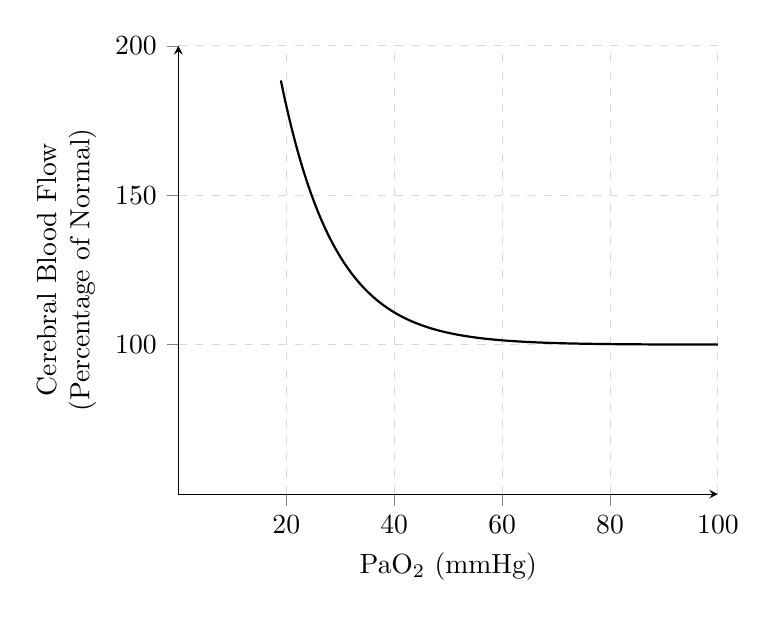
\begin{tikzpicture}


\begin{axis}[
        axis lines=middle,
        grid = major,
        grid style={dashed, gray!30},
	ymin = 50,
	ymax = 200,
	xmin = 0,
	xmax =100,
	 ylabel near ticks,
	xlabel near ticks,
        xlabel=PaO\textsubscript{2} (mmHg),
        ylabel=Cerebral Blood Flow \\ (Percentage of Normal),
        tick align=outside,
        enlargelimits=false,
ylabel style={align=center},
legend pos= north west,
legend style={font=\small, cells={align=left}}]

	\addplot[domain=19:100, black, thick,samples=500] {100+80*e^(-0.1*(x-20))};

\end{axis}

\end{tikzpicture} 
\end{document}